\documentclass[tikz,border=2pt]{standalone}
\usepackage{amsmath}
\usepackage{amssymb}
\usepackage{xcolor}

\definecolor{journalink}{HTML}{1F1C18}
\definecolor{journalmuted}{HTML}{8A7F72}
\definecolor{journalaccent}{HTML}{9C2D2D}

\begin{document}
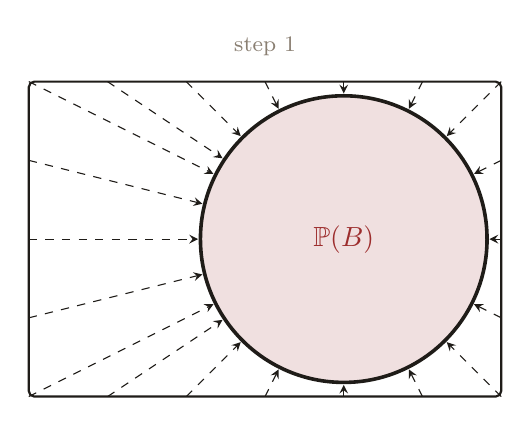
\begin{tikzpicture}[
  x=1cm,
  y=1cm,
  every node/.style={font=\normalsize},
  >=stealth
]
  \def\circleB{(2,0) circle (1.82)}
  \begin{scope}
    \path[fill=journalaccent, fill opacity=0.15] \circleB;
  \end{scope}
  \draw[journalink, line width=0.8pt, rounded corners=2pt] (-2,-2) rectangle (4,2);
  \draw[journalink, line width=1.3pt] \circleB;
  \node[journalaccent] at (2,0) {$\mathbb{P}(B)$};
  \node[journalmuted] at (1,2.45) {\footnotesize step 1};

  \draw[journalink, dashed, ->] (-2,-2) -- (0.3453097,-0.8273452);
  \draw[journalink, dashed, ->] (-1,-2) -- (0.460707,-1.026195);
  \draw[journalink, dashed, ->] (0,-2) -- (0.6918525,-1.3081475);
  \draw[journalink, dashed, ->] (1,-2) -- (1.172655,-1.654690);
  \draw[journalink, dashed, ->] (2,-2) -- (2,-1.85);
  \draw[journalink, dashed, ->] (3,-2) -- (2.827345,-1.654690);
  \draw[journalink, dashed, ->] (4,-2) -- (3.308148,-1.308148);
  \draw[journalink, dashed, ->] (-2,-1) -- (0.2052364,-0.4486909);
  \draw[journalink, dashed, ->] (4,-1) -- (3.6546903,-0.8273452);
  \draw[journalink, dashed, ->] (-2,0) -- (0.15,0);
  \draw[journalink, dashed, ->] (4,0) -- (3.85,0);
  \draw[journalink, dashed, ->] (-2,2) -- (0.3453097,0.8273452);
  \draw[journalink, dashed, ->] (-1,2) -- (0.460707,1.026195);
  \draw[journalink, dashed, ->] (0,2) -- (0.6918525,1.3081475);
  \draw[journalink, dashed, ->] (1,2) -- (1.172655,1.654690);
  \draw[journalink, dashed, ->] (2,2) -- (2,1.85);
  \draw[journalink, dashed, ->] (3,2) -- (2.827345,1.654690);
  \draw[journalink, dashed, ->] (4,2) -- (3.308148,1.308148);
  \draw[journalink, dashed, ->] (-2,1) -- (0.2052364,0.4486909);
  \draw[journalink, dashed, ->] (4,1) -- (3.6546903,0.8273452);
\end{tikzpicture}
\end{document}
